%%
%% This is file `leaflet-manual.tex',
%% generated with the docstrip utility.
%%
%% The original source files were:
%%
%% leaflet.dtx  (with options: `manual')
%%
%% Copyright (C) 2003, 2004
%% Rolf Niepraschk, Rolf.Niepraschk@ptb.de
%% Hubert Gaesslein, HubertJG@open.mind.de
%%
%% This work may be distributed and/or modified under the
%% conditions of the LaTeX Project Public License, either version 1.3
%% of this license or (at your option) any later version.
%% The latest version of this license is in
%%   http://www.latex-project.org/lppl.txt
%% and version 1.3 or later is part of all distributions of LaTeX
%% version 2003/12/01 or later.
%%
%% This work has the LPPL maintenance status "author-maintained".
%%
\def\filename{leaflet-manual.tex}
\def\fileversion{v1.0d}   % change this when leaflet-manual changed, too.
\def\filedate{2012/06/04}
\def\docdate {2012/06/04} % change this when leaflet-manual changed, too.
\listfiles
\errorcontextlines=99
\documentclass[
%%notumble,
%%nofoldmark,
%%dvipdfm,
%%portrait,
%%titlepage,
%%nocombine,
%%a3paper,
%%debug,
%%nospecialtricks,
%%draft,
]{leaflet}


\renewcommand*\foldmarkrule{.3mm}
\renewcommand*\foldmarklength{5mm}

\usepackage[T1]{fontenc}
\usepackage{textcomp}
\usepackage{mathptmx}
\usepackage[scaled=0.9]{helvet}
\makeatletter
\def\ptmTeX{T\kern-.1667em\lower.5ex\hbox{E}\kern-.075emX\@}
\DeclareRobustCommand{\ptmLaTeX}{L\kern-.3em
        {\setbox0\hbox{T}%
         %\vb@xt@ % :-)
         \vbox to\ht0{\hbox{%
                            \csname S@\f@size\endcsname
                            \fontsize\sf@size\z@
                            \math@fontsfalse\selectfont
                            A}%
                      \vss}%
        }%
        \kern-.12em
        \ptmTeX}
\makeatother
\let\TeX=\ptmTeX
\let\LaTeX=\ptmLaTeX
\usepackage{shortvrb}
\MakeShortVerb{\|}
\usepackage{url}
\usepackage{graphicx}
\usepackage[dvipsnames,usenames]{color}
\usepackage{listings}
\definecolor{LIGHTGRAY}{gray}{.9}

%%%%\renewcommand{\descfont}{\normalfont}
\newcommand\Lpack[1]{\textsf{#1}}
\newcommand\Lclass[1]{\textsf{#1}}
\newcommand\Lopt[1]{\texttt{#1}}
\newcommand\Lprog[1]{\textit{#1}}

\newcommand*\defaultmarker{\textsuperscript\textasteriskcentered}

\title{Processing Fundamentals\vspace{-2ex}}
\author{%
  Dan Lidral-Porter\vspace{-2ex}
}
\date{}

\CutLine*{1}
\CutLine*{6}

%AddToBackground{5}{%  Background of a small page
% \put(0,0){\textcolor{Cerulean}{\rule{\paperwidth}{\paperheight}}}}
%
%AddToBackground*{2}{% Background of a large page
% \put(\LenToUnit{.5\paperwidth},\LenToUnit{.5\paperheight}){%
%   \makebox(0,0)[c]{%
%     \resizebox{.9\paperwidth}{!}{\rotatebox{35.26}{%
%       \textsf{\textbf{\textcolor{LIGHTGRAY}{BACKGROUND}}}}}}}}

\begin{document}

\definecolor{framegrey}{rgb}{0.7,0.7,0.7}

\lstset{language=Java
       ,basicstyle=\ttfamily
       ,frame=single
       ,rulecolor=\color{framegrey}
       }

\maketitle
\thispagestyle{empty}

%%\LARGE

\section{Code Terminology}

Processing artworks are called \textit{sketches}.
You enter code for your sketch in the large white section of the Processing IDE (the \textit{editor area}).

A sktech is a series of statements.
Each statement in the code is terminated by a semicolon.
A statement typically involves using a \textit{function} by \textit{calling} it.
When you \textit{call} a function, you add parentheses after its name, and in between this you give a comma-seperated list of values.
Each such value is called an \textit{argument} of the function.

\begin{lstlisting}
println("hello", "world!");
\end{lstlisting}
\vspace{-0.5em}
This statement calls the \texttt{println} function with two arguments, \texttt{"hello"} and \texttt{"world!"}.
The \texttt{println} function causes text to appear at the bottom of the Processing IDE, in the \textit{console area}.
It forms a complete sketch by itself; try entering it in your editor area and running it.

\textbf{Exercise 1.1:} see what happens when you remove the semicolon from the \texttt{println} statement.

When your sketch has an error such as a missing semicolon, the IDE's \textit{message line} turns yellow and displays the best error message it can.

Lines that start with two forward slashes (\texttt{//}) are comments.
Processing ignores them so you can leave notes.

\vspace{-0.5em}

\section{The Canvas}

Every sketch begins by defining the size of the window it will use, called the \textit{canvas}.

The \texttt{size} function is used to define the size of the canvas, in pixels.
The general form of the size function is \texttt{size(width, height)}.
The values for width and height must be whole numbers (no decimal points).

Here's an example:

\begin{lstlisting}
size(1280, 720);
\end{lstlisting}

This creates a canvas that is 1280 pixels wide and 720 pixels high.
Try creating a sketch with only a size function, and change the numbers to experiment with the width and height.

A location within the canvas is described using two numbers, called the \textit{coordinates}.
This figure illustrates the names of the coordinates:

\begin{figure}[!h]
  \centering
  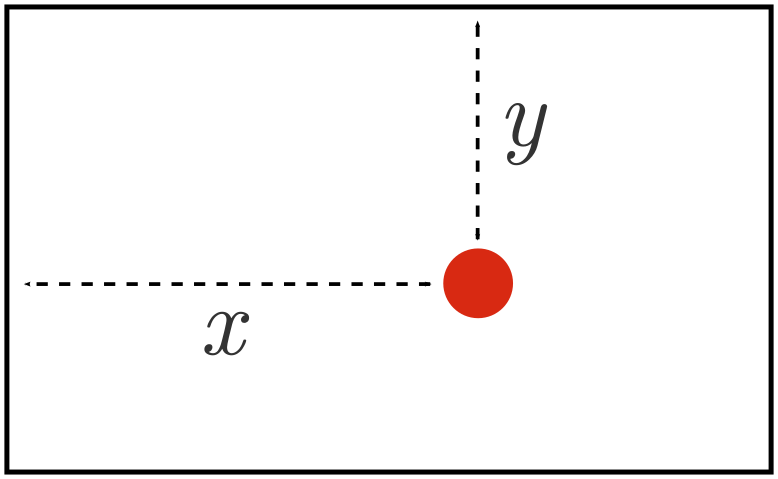
\includegraphics[scale=.25]{canvas.eps}
\end{figure}

Coordinates are displayed as \texttt{(x, y)}, where \texttt{x} is the x-coordinate, and \texttt{y} is the y-coordinate.

\textbf{Exercise 1.2:} where would the red dot be if the x-coordinate were zero?
What about the y-coordinate?
What about both?

\section{Color}

Computers store colors as amount of red, green, and blue light, but this is hard to reason about.
A more natural way of representing colors is with \textit{hue}, \textit{saturation}, and \textit{brightness}.

The \textit{hue} is the base coloring of the color, before it's modified by the saturation and brightness values.
The hue starts and ends at red, and in between covers the whole color wheel.

The \textit{saturation} is how strong the color is.
Full saturation means the color is as intensely colored as possible.
A saturation of zero produces values of grey.

The \textit{brightness} is how much light the color emits.
A brightness of zero means the color is black, no matter what the other values.

\textbf{Exercise 1.3:} consider pure white. What is its brightness? How about its saturation? Does its hue matter?

You can tell Processing to use hue, saturation, and brightness by using the \texttt{colorMode} function:

\begin{lstlisting}
colorMode(HSB, 100);
\end{lstlisting}

The \texttt{HSB} means you want to use Hue, Saturation, and Brightness mode, and the \texttt{100} means that you want the maximum value for each to be 100.
You should put this in a sketch right after the \texttt{size} function.

After the \texttt{colorMode} function, you can create colors by using the \texttt{color} function.
The general form of the color function is \texttt{color(hue, saturation, brightness)}.

A simple thing to use colors with is the \texttt{background} function, which paints the entire canvas with the color you give it.
Here is a sketch that paints the whole canvas yellow using the \texttt{background} function:

\begin{lstlisting}
size(1280, 720);
colorMode(HSB, 100);
background( color(14, 100, 90) );
\end{lstlisting}

\textbf{Exercise 1.4:} write a sketch that paints the canvas purple.

\section{Shapes}

Enough with flat colors, let's draw some shapes!

Every two-dimensional shape in Processing can have one of two visual attributes: the \textit{stroke}, which is the color of its outline, and the \textit{fill}, which is the interior color.

The stroke color is set with the \texttt{stroke} function, which takes a color.
The stroke has a thickness, called the \textit{weight}.
It is set by the \texttt{strokeWeight} function, which takes a number in pixels.
The stroke can be turned off by using the \texttt{noStroke} function, which doesn't take anything.
(You still need to use the parentheses, like this: `\texttt{noStroke();}'.)

The fill color is set by the \texttt{fill} function, which takes only a color.
It can be turned off by using the \texttt{noFill} function, which takes nothing.

The three shapes that are both simple and easy to draw with Processing are circles, lines, and rectangles.

Circles are drawn with the \texttt{ellipse} function, since circles are just a special case of ellipses.
To draw a circle, the last two arguments to the ellipse (how wide \& tall it is) are always the same.
The general form of the "circle" function is then \texttt{ellipse(x, y, r, r)} where \textit{x} is the x-coordinate, \textit{y} is the y-coordinate, and \textit{r} is the radius.

\textbf{Exercise 1.5:} draw a circle in the middle of a blue canvas that has green stroke and orange fill.

Lines have no fill, just a stroke.
The line function looks like \texttt{line(x1, y1, x2, y2)}.
The first two values are the \textit{x} and \textit{y} coordinates of the first point, and the second two are the coordinates of the second point.

\textbf{Exercise 1.6:} using lines, draw a big "x" across a canvas.

Rectangles are made with the \texttt{rect} function.
Its general form is \texttt{rect(x, y, w, h)}, where \textit{x} and \textit{y} are the coordinates of the upper-left corner of the rectangle, and \textit{w} and \textit{h} are how wide and tall it is, respectively.

\textbf{Exercise 1.7:} cover a canvas with four colored rectangles.

If you are having difficulty with the exercises, it may be helpful to start with the "All Together" sketch below and experiment with it until you arrive upon the solution.

\section{All Together}

Here is a sketch that draws a circle, a rectangle, and two horizontal lines, all with the same stroke and fill:

\begin{lstlisting}
size(1280, 720);
colorMode(HSB, 100);
background( color(0, 0, 83) );

stroke( color(7, 88, 77) );
strokeWeight(20);
fill( color(20, 77, 32) );

ellipse(300, 200, 175, 175);
rect(450, 75, 600, 300);

line(215, 430, 1060, 430);
line(215, 480, 1060, 480);
\end{lstlisting}


\section{Cheatsheet}

\texttt{size(width, height)} - width and height should be numbers in pixels.

\texttt{colorMode(HSB, 100)} - tell Processing to use hue, saturation, and brightness color mode with a maximum of 100.

\texttt{color(hue, saturation, brightness)} - create the color with the given attributes (numbers up to 100).
Must be used after the \texttt{colorMode} function above.

\texttt{background(color)} - paint the entire canvas a specific color.

\texttt{stroke(color)} - set the color of shape outlines.

\texttt{strokeWeight(thickness)} - set the width of shape outlines, in pixels.

\texttt{noStroke()} - turn off shape outlines.

\texttt{fill(color)} - set the color of the insides of shapes.

\texttt{noFill()} - turn off coloring inside of shapes.

\texttt{ellipse(x, y, rw, rh)} - draw an ellipse centered at \texttt{(x, y)}, with width \texttt{rw} and height \texttt{rh}.
For a circle, have \texttt{rw} and \texttt{rh} be the same.

\texttt{rect(x, y, w, h)} - draw a rectangle whose upper-left corner is at \texttt{(x, y)} and has width \texttt{w} and height \texttt{h}.

\texttt{line(x1, y1, x2, y2)} - draw a line from coordinates \texttt{(x1, y1)} to \texttt{(x2, y2)}.
(Its thickness will be the current stroke weight.)


\begin{thebibliography}{000}
\bibitem{cit:processing-ref}
  \textsc{B. Fry, C. Reas, et. al.}: The Processing Language Reference. 2001-\\
  \url{http://processing.org/reference}
\end{thebibliography}

\loggingall
\end{document}
\endinput
%%
%% End of file `leaflet-manual.tex'.
